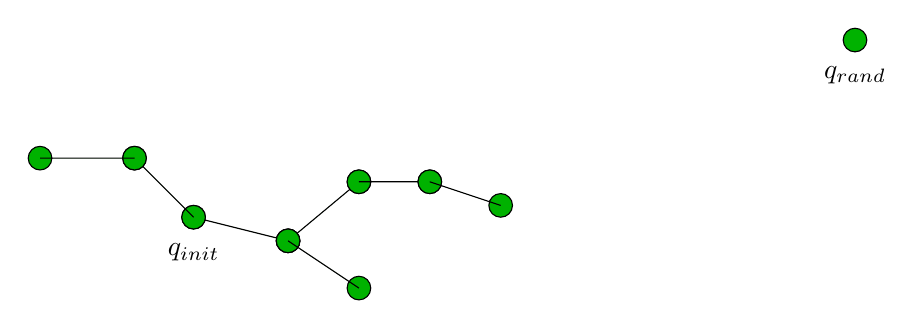
\begin{tikzpicture}[scale=1.5]
\draw [fill=black!30!green] (0,0) circle [radius =0.1] -- (0.8,-0.2) circle [radius =0.1];
\draw [fill=black!30!green] (0,0) circle [radius =0.1] -- (-0.5,0.5) circle [radius =0.1];
\node [] at (0,-0.3) {$q_{\text{init}}$};
\draw [fill=black!30!green] (-0.5,0.5) circle [radius =0.1] -- (-1.3,0.5) circle [radius =0.1];
\draw [fill=black!30!green] (0.8,-0.2) circle [radius =0.1] -- (1.4,0.3) circle [radius =0.1];
\draw [fill=black!30!green] (0.8,-0.2) circle [radius =0.1] -- (1.4,-0.6) circle [radius =0.1];
\draw [fill=black!30!green] (1.4,0.3) circle [radius =0.1] -- (2,0.3) circle [radius =0.1]; % criar no a partir dele para começar a explicar

\draw [fill=black!30!green] (2,0.3) circle [radius =0.1] -- (2.6,0.1) circle [radius =0.1]; % q_near
% \node [] at (2.6,-0.2) {$q_{\text{near}}$};
\draw [fill=black!30!green] (5.6,1.5) circle [radius =0.1]; 
\node [] at (5.6,1.2) {$q_{\text{rand}}$};

\end{tikzpicture}
